\documentclass[a4paper,14pt]{extarticle} % the default article class is limited to 12pt, but you can go up to 14, 17 or 20 points if you use the extarticle class:
\usepackage{cmap} % make LaTeX PDF output copy-and-pasteable
\usepackage[T2A]{fontenc}
\usepackage[utf8]{inputenc}
\usepackage[english,ukrainian]{babel}

\usepackage{amssymb,amsfonts,mathtools,amsmath,cite,enumerate,float}
\usepackage{indentfirst} % set an additional space before a paragraph at the begining of new section
\usepackage{setspace}
\usepackage{textcomp}

\usepackage{import} % for adding a file by path https://tex.stackexchange.com/questions/246/when-should-i-use-input-vs-include

\usepackage{geometry} 
\geometry{left=1.25cm}
\geometry{right=1.25cm}
\geometry{top=1cm}
\geometry{bottom=2cm}

\usepackage[table,xcdraw,dvipsnames]{xcolor}
\usepackage{color}
% 1) tutorial about xcolor:  https://www.overleaf.com/learn/latex/Using_colours_in_LaTeX
% 2) huge tutorial about xcolor: https://latex-tutorial.com/color-latex/ 
% 3) RGB calculator: https://www.w3schools.com/colors/colors_rgb.asp

\usepackage{hyperref}
\definecolor{linkcolor}{HTML}{0000FF}
\definecolor{urlcolor}{HTML}{0000FF} 
\hypersetup{pdfstartview=FitH, linkcolor=linkcolor, urlcolor=urlcolor, colorlinks=true}

\usepackage{graphicx}
\usepackage{wrapfig}
\graphicspath{{Screenshots/}} % path to images

\parskip=1mm %space between paragraphs

\usepackage{listingsutf8} % for code (origin: \usepackage{listings})

\lstset{
    frame=single, %lines
    language=Python,
    aboveskip=3mm,
    belowskip=3mm,
    columns=flexible,
    basicstyle={\small\ttfamily},
    numbers=left,
    numberstyle=\tiny\color{gray},
    commentstyle=\color{OliveGreen},
    stringstyle=\color{Mahogany},
    morestring=[b]''',
    showstringspaces=false,
    keywordstyle=\bfseries\color{blue},
    emph={[1]import, as, for, return}, emphstyle={[1]\bfseries\color{magenta}},
    emph={[2]range}, emphstyle={[2]\bfseries\color{brown}},
    breaklines=true,
    breakatwhitespace=true,
    tabsize=4,
    extendedchars=false, % to use ukrainian text in a code
    inputencoding=utf8 % to use ukrainian text in a code
}

\begin{document}

\section*{Додаткове завдання до Лабораторної роботи \textnumero4}

\textbf{Завдання:} Модифікувати функцію \texttt{create\_instance()} так, щоб у новостворений інстанс одразу 
скопіювалися файли з git-репозиторію.

\textbf{Виконання:} Основна ідея полягає у запуску через код Python двох термінальних команд за допомогою 
\texttt{os.system()}:
\begin{enumerate}
    \item Команда \texttt{pscp} копіювання bash-скрипту на інстанс, де bash-скрипт містить рядки встановлення 
    \texttt{git} та клонування файлів \texttt{git clone};
    \item Команда створення \texttt{ssh} тунелю та запуску щойно перенесеного на інстанс bash-скрипту; 
\end{enumerate}

Створивши завчасно нову пару ключів з назвою <<pair5>>, а також два відповідних файли 
<<pair5.pem>> та <<pair5.ppk>>, можемо запускати модифіковану функцію \texttt{create\_instance()}:

\lstinputlisting[firstnumber=1, firstline=15, lastline=52, label = create instance, caption = Створення інстансу]{os.py}

У коді зроблено важливі зауваження: по-перше, при створенні інстансу необхідно вказати ім'я 
<<SecurityGroupIds>>, інакше цей параметр буде заданий по замовчуванню, що не дозволить у подальшому виконати 
\texttt{ssh}-тунель. По-друге, власне при спробі створення \texttt{ssh}-тунелю необхідно одразу виконати наступну 
команду \texttt{bash commands.sh} (тобто ще до відключення). Реалізується це за схемою:
\[ \texttt{ssh -t ubuntu@domain 'bash commands.sh; bash'} \]

Ну і наостанок самі команди у bash-скрипті:

\begin{lstlisting}[language=bash, stringstyle=\small\ttfamily, emphstyle={[1]\small\ttfamily}]
    #!/bin/bash

    sudo apt update
    sudo apt install git
    git clone https://github.com/Tom-Paxter/AWS_laboratory.git
    
\end{lstlisting}

І самі зображення (Рис. 1 довелося зменшити, щоб втиснувся на сторінку...).

\begin{figure}[H]
    \center{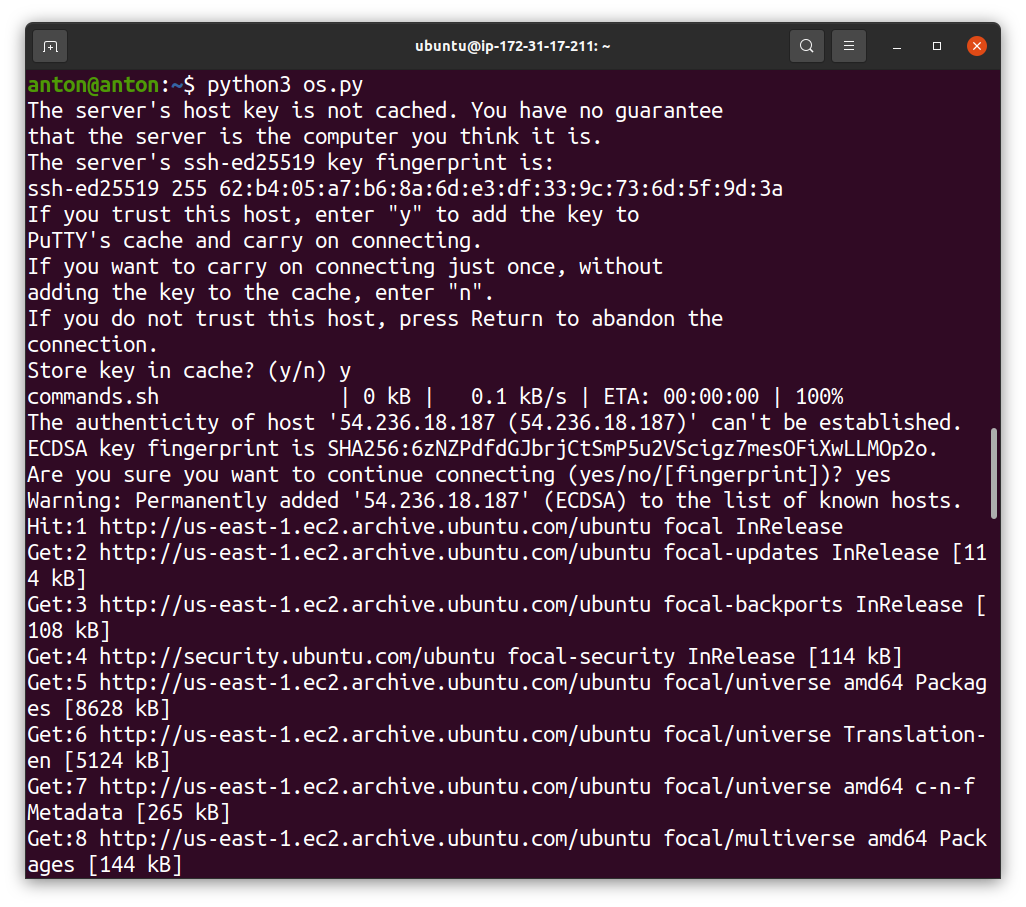
\includegraphics[width=0.7\linewidth]{1.png}}
    \caption{Запуск файлу \texttt{os.py}}
    \label{fig:1}
\end{figure}

\begin{figure}[H]
    \center{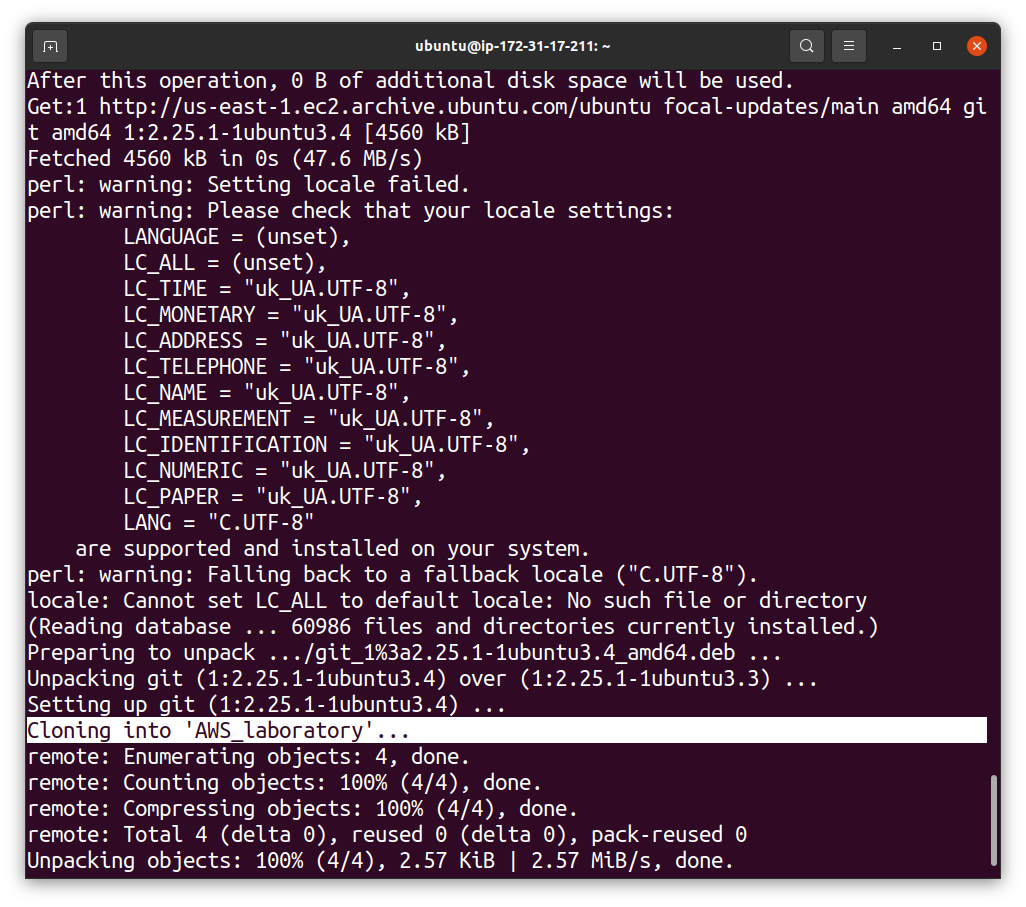
\includegraphics[width=1\linewidth]{2.png}}
    \caption{Завершення виконання}
    \label{fig:2}
\end{figure}

\begin{figure}[H]
    \center{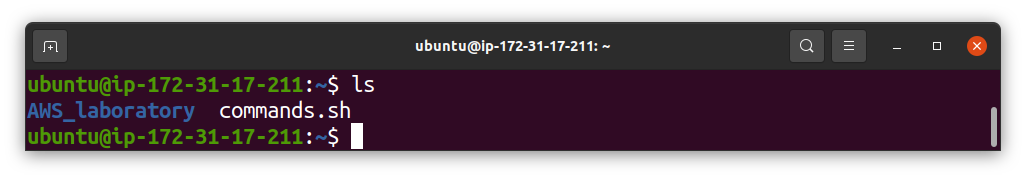
\includegraphics[width=1\linewidth]{3.png}}
    \caption{Перевірка результатів}
    \label{fig:3}
\end{figure}

\end{document}